\documentclass[aspectratio=169]{beamer}

% ── Base theme ──────────────────────────────────────────────────────────────
\usetheme{Madrid}
\setbeamertemplate{navigation symbols}{}

% ── Brand colors ─────────────────────────────────────────────────────────────
\definecolor{fptOrange}{HTML}{F37021}
\definecolor{fptNavy}{HTML}{1A2B4A}
\definecolor{fptLight}{HTML}{FFF5EE}
\definecolor{positive}{HTML}{0173B2}
\definecolor{negative}{HTML}{DE8F05}
\definecolor{emphasis}{HTML}{029E73}
\definecolor{neutral}{gray}{0.55}
\definecolor{cbPurple}{HTML}{CC78BC}

% ── Color palette ────────────────────────────────────────────────────────────
\setbeamercolor{palette primary}{bg=fptNavy,fg=white}
\setbeamercolor{palette secondary}{bg=fptNavy!80,fg=white}
\setbeamercolor{palette tertiary}{bg=fptOrange,fg=white}
\setbeamercolor{palette quaternary}{bg=fptNavy,fg=white}
\setbeamercolor{structure}{fg=fptOrange}
\setbeamercolor{frametitle}{bg=fptNavy,fg=white}
\setbeamercolor{title}{bg=fptNavy,fg=white}
\setbeamercolor{subtitle}{fg=fptOrange}
\setbeamercolor{section in toc}{fg=fptNavy}
\setbeamercolor{normal text}{fg=fptNavy}
\setbeamercolor{block title}{bg=fptNavy!10,fg=fptNavy}
\setbeamercolor{block body}{bg=fptNavy!4,fg=fptNavy}
\setbeamercolor{block title alerted}{bg=fptOrange!20,fg=fptOrange!80!black}
\setbeamercolor{block body alerted}{bg=fptOrange!6,fg=fptNavy}
\setbeamercolor{block title example}{bg=emphasis!15,fg=emphasis!70!black}
\setbeamercolor{block body example}{bg=emphasis!4,fg=fptNavy}

% ── Fonts ────────────────────────────────────────────────────────────────────
\usepackage{fontspec}
\setbeamerfont{title}{size=\Large,series=\bfseries}
\setbeamerfont{subtitle}{size=\normalsize,series=\normalfont}
\setbeamerfont{frametitle}{size=\large,series=\bfseries}
\setbeamerfont{block title}{size=\normalsize,series=\bfseries}

% ── Packages ─────────────────────────────────────────────────────────────────
\usepackage{amsmath,amssymb,booktabs,array}
\usepackage{graphicx}
\usepackage{tikz}
\usetikzlibrary{arrows.meta,positioning,shapes.geometric,automata}
\usepackage{eso-pic}

% ── Kill Madrid's section headline bars ──────────────────────────────────────
\setbeamertemplate{headline}{}

% ── Frametitle with logo ──────────────────────────────────────────────────────
\setbeamertemplate{frametitle}{%
  \nointerlineskip%
  \begin{beamercolorbox}[wd=\paperwidth,ht=1.1cm,dp=0.2cm,leftskip=8pt,rightskip=8pt]{frametitle}%
    \usebeamerfont{frametitle}\color{white}\insertframetitle%
    \hfill%
    
\includegraphics[height=0.88cm]{../../docs/logo/fpt_logo.png}%
  \end{beamercolorbox}%
  \begin{beamercolorbox}[wd=\paperwidth,ht=2pt,dp=0pt]{palette tertiary}%
  \end{beamercolorbox}%
}

% ── Custom footline ───────────────────────────────────────────────────────────
\setbeamertemplate{footline}{%
  \leavevmode%
  \begin{beamercolorbox}[wd=\paperwidth,ht=2.5ex,dp=1.2ex,leftskip=8pt,rightskip=8pt]{palette primary}%
    \usebeamerfont{footline}\footnotesize
    \insertshortauthor\hfill
    \insertshorttitle\hfill
    \insertframenumber\,/\,\inserttotalframenumber\hspace{4pt}
  \end{beamercolorbox}%
}

\newcommand{\pos}[1]{\textcolor{positive}{#1}}
\newcommand{\con}[1]{\textcolor{negative}{#1}}
\newcommand{\HL}[1]{\textcolor{emphasis}{#1}}

\newcommand{\backupbegin}{%
  \newcounter{framenumberappendix}%
  \setcounter{framenumberappendix}{\value{framenumber}}%
}
\newcommand{\backupend}{%
  \addtocounter{framenumberappendix}{-\value{framenumber}}%
  \addtocounter{framenumber}{\value{framenumberappendix}}%
}

\title[Vietnamese GraphRAG --- Multi-hop QA]{Vietnamese GraphRAG\\Multi-hop Question Answering over Wikipedia}
\subtitle{Capstone Review 2 --- FPT University SE+AI}
\author[Trung, Anh, Khoi, Thien]{%
  Huynh Quoc Trung (QE180038) \and
  Nhu Quang Anh (QE180005) \and
  Pham Ngo Dinh Khoi (QE180110) \and
  Truong Dinh Thien (QE180018)
}
\institute{FPT University\\[4pt]\small\textit{Supervisors:} Lê Trung Hiếu \quad Đặng Nguyên Bình}
\date{Week 8 --- July 2026}

\begin{document}

% ── SLIDE 1: Title ────────────────────────────────────────────────────────────
\begin{frame}[plain]
\titlepage
\end{frame}

% ── SLIDE 2: Table of Contents ────────────────────────────────────────────────
\begin{frame}{Table of Contents}
\begin{columns}[T]
\column{0.48\textwidth}
\begin{enumerate}
  \item System Architecture
  \item Deployment \& Configuration
  \item Ingestion \& Query Dataflow
  \item Graph Schema (ERD)
  \item Physical Design
  \item Job State Machine
  \item Screen Design
\end{enumerate}
\column{0.48\textwidth}
\begin{enumerate}
  \setcounter{enumi}{7}
  \item Technology Choices
  \item Coding Quality \& Patterns
  \item Algorithm Complexity
  \item Data Pipeline (Corpus Filtering)
  \item Data Pipeline (Schema v0.4)
  \item Data Pipeline (Reasoning Types)
  \item Data Pipeline (QA \& QC)
  \item Model Training
  \item Evaluation Results
  \item Team \& Timeline
\end{enumerate}
\end{columns}
\end{frame}

% ── SLIDE 3: System Architecture ─────────────────────────────────────────────
\begin{frame}{1. System Architecture}
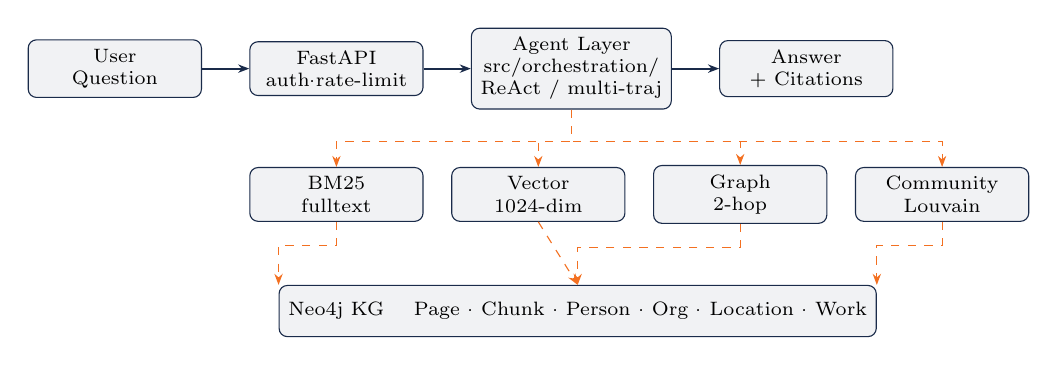
\begin{tikzpicture}[
  box/.style={draw=fptNavy,rounded corners=3pt,fill=fptNavy!6,
              minimum width=2.2cm,minimum height=0.65cm,font=\scriptsize,align=center},
  arr/.style={-{Stealth[length=4pt]},fptNavy,thick},
  darr/.style={-{Stealth[length=4pt]},fptOrange,dashed},
  node distance=0.45cm and 0.5cm
]
  % Row 1
  \node[box] (user)  {User\\Question};
  \node[box,right=0.6cm of user]  (api)   {FastAPI\\auth·rate-limit};
  \node[box,right=0.6cm of api]   (agent) {Agent Layer\\src/orchestration/\\ReAct / multi-traj};
  \node[box,right=0.6cm of agent] (ans)   {Answer\\+ Citations};

  \draw[arr] (user) -- (api);
  \draw[arr] (api)  -- (agent);
  \draw[arr] (agent) -- (ans);

  % Row 2 — retrieval signals
  \node[box,below=0.9cm of api]   (bm25) {BM25\\fulltext};
  \node[box,right=0.35cm of bm25] (vec)  {Vector\\1024-dim};
  \node[box,right=0.35cm of vec]  (grph) {Graph\\2-hop};
  \node[box,right=0.35cm of grph] (comm) {Community\\Louvain};

  \draw[darr] (agent.south) -- ++(0,-0.4) -| (bm25.north);
  \draw[darr] (agent.south) -- ++(0,-0.4) -| (vec.north);
  \draw[darr] (agent.south) -- ++(0,-0.4) -| (grph.north);
  \draw[darr] (agent.south) -- ++(0,-0.4) -| (comm.north);

  % Row 3 — Neo4j
  \node[box,below=0.8cm of vec,xshift=0.5cm,minimum width=5.8cm] (neo4j)
        {Neo4j KG \quad Page · Chunk · Person · Org · Location · Work};

  \draw[darr] (bm25.south) -- ++(0,-0.3) -| (neo4j.north west);
  \draw[darr] (vec.south)  -- (neo4j.north);
  \draw[darr] (grph.south) -- ++(0,-0.3) -| (neo4j.north);
  \draw[darr] (comm.south) -- ++(0,-0.3) -| (neo4j.north east);
\end{tikzpicture}

\vspace{2pt}
{\scriptsize Deployment: systemd Neo4j 5.x · uvicorn FastAPI · Python 3.12 · local GPU}
\end{frame}

% ── SLIDE 4: Deployment & Configuration ──────────────────────────────────────
\begin{frame}[shrink=5]{2. Deployment \& Configuration}
\begin{columns}[T]
\column{0.50\textwidth}
\begin{tabular}{@{}lll@{}}
\toprule
\textbf{Component} & \textbf{Runtime} & \textbf{Start Command} \\
\midrule
Neo4j 5.x   & systemd  & \texttt{\scriptsize sudo systemctl start neo4j} \\
FastAPI     & uvicorn  & \texttt{\scriptsize uv run uvicorn src.main:app} \\
Gradio Demo & Python   & \texttt{\scriptsize uv run python src/app\_gradio.py} \\
MCP Server  & Python   & \texttt{\scriptsize uv run python -m src.mcp\_pkg} \\
\bottomrule
\end{tabular}

\column{0.46\textwidth}
\begin{exampleblock}{All config via pydantic-settings}
\begin{itemize}\setlength\itemsep{1pt}\scriptsize
  \item \texttt{NER\_BACKEND} (simple/underthesea/wikilink/\ldots)
  \item \texttt{EMBEDDING\_BACKEND} (gemini/local)
  \item \texttt{MODEL\_MODE} (api/local)
  \item \texttt{WRRF\_WEIGHT\_BM25/VECTOR/GRAPH}
  \item \texttt{AGENT\_N\_TRAJECTORIES}
  \item \texttt{NEO4J\_URI} / \texttt{APP\_API\_KEY}
\end{itemize}
\smallskip
\textit{Zero hard-coded credentials --- \texttt{.env.example} provided}
\end{exampleblock}
\end{columns}
\end{frame}

% ── SLIDE 5: Ingestion & Query Dataflow ──────────────────────────────────────
\begin{frame}{3. Ingestion \& Query Dataflow}
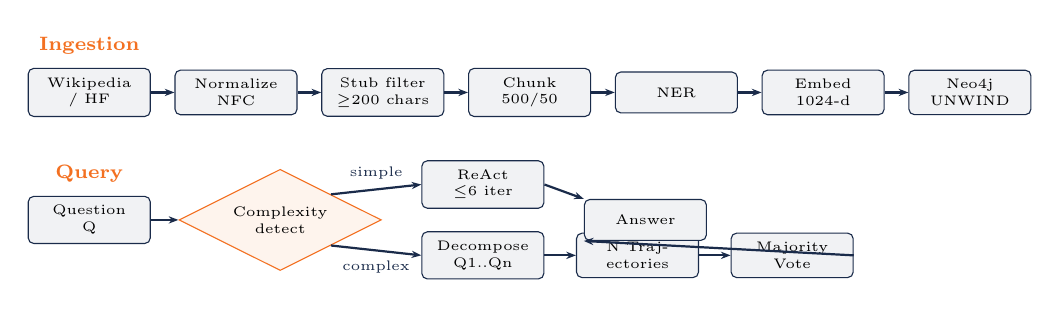
\begin{tikzpicture}[
  proc/.style={draw=fptNavy,fill=fptNavy!6,rounded corners=2pt,
               minimum width=1.55cm,minimum height=0.52cm,font=\tiny,align=center},
  dec/.style={draw=fptOrange,fill=fptOrange!8,diamond,aspect=2,
              minimum width=1.6cm,minimum height=0.45cm,font=\tiny,align=center},
  arr/.style={-{Stealth[length=3.5pt]},fptNavy,thick},
  node distance=0.25cm and 0.3cm
]
  % ── Ingestion pipeline (top row) ──────────────────────────────────────────
  \node[proc] (src)   {Wikipedia\\/ HF};
  \node[proc,right=0.3cm of src]  (nfc)   {Normalize\\NFC};
  \node[proc,right=0.3cm of nfc]  (stub)  {Stub filter\\ $\geq$200 chars};
  \node[proc,right=0.3cm of stub] (chunk) {Chunk\\500/50};
  \node[proc,right=0.3cm of chunk](ner)   {NER};
  \node[proc,right=0.3cm of ner]  (emb)   {Embed\\1024-d};
  \node[proc,right=0.3cm of emb]  (neo)   {Neo4j\\UNWIND};

  \draw[arr] (src)--(nfc); \draw[arr] (nfc)--(stub); \draw[arr] (stub)--(chunk);
  \draw[arr] (chunk)--(ner); \draw[arr] (ner)--(emb); \draw[arr] (emb)--(neo);

  \node[above=0.05cm of src,font=\scriptsize\bfseries,fptOrange] {Ingestion};

  % ── Query pipeline (bottom rows) ──────────────────────────────────────────
  \node[proc,below=1.0cm of src]        (q)    {Question\\Q};
  \node[dec, right=0.35cm of q]         (cpx)  {Complexity\\detect};
  \node[proc,right=0.5cm of cpx,yshift= 0.45cm] (reac) {ReAct\\$\leq$6 iter};
  \node[proc,right=0.5cm of cpx,yshift=-0.45cm] (dec)  {Decompose\\Q1..Qn};
  \node[proc,right=0.4cm of dec]        (traj) {N Traj-\\ectories};
  \node[proc,right=0.4cm of traj]       (vote) {Majority\\Vote};
  \node[proc,right=0.5cm of reac,yshift=-0.45cm] (ansq) {Answer};

  \draw[arr] (q)--(cpx);
  \draw[arr] (cpx.north east) -- node[above,font=\tiny]{simple} (reac.west);
  \draw[arr] (cpx.south east) -- node[below,font=\tiny]{complex} (dec.west);
  \draw[arr] (dec)--(traj); \draw[arr] (traj)--(vote);
  \draw[arr] (reac.east) -- (ansq.north west);
  \draw[arr] (vote.east) -- (ansq.south west);

  \node[above=0.05cm of q,font=\scriptsize\bfseries,fptOrange] {Query};
\end{tikzpicture}
\end{frame}

% ── SLIDE 6: Graph Schema (ERD) ───────────────────────────────────────────────
\begin{frame}[shrink=5]{4. Graph Schema (ERD)}
\begin{columns}[T]
\column{0.52\textwidth}
{\ttfamily\scriptsize
\begin{itemize}\setlength\itemsep{2pt}
  \item (\textcolor{fptOrange}{:Page} \{id, title, url, text, source\})
  \item (\textcolor{fptOrange}{:Chunk} \{id, text, embedding[1024], seq\_num, page\_id\})
  \item (\textcolor{fptOrange}{:Person/:Org/:Location/:Work} \{id, name, aliases[]\})
  \item (\textcolor{fptOrange}{:Community} \{id, level, summary, member\_ids[]\})
\end{itemize}
}
\smallskip
{\scriptsize
\textbf{Edges:} \texttt{HAS\_CHUNK}, \texttt{MENTIONS\_*}, \texttt{LINKS\_TO}

\textbf{Relations:} \texttt{FOUNDED\_BY}, \texttt{LOCATED\_IN}, \texttt{BORN\_IN},
\texttt{MEMBER\_OF}, \texttt{PART\_OF}, \texttt{CREATED\_BY}
}

\column{0.44\textwidth}
\begin{block}{Constraints (UNIQUE)}
{\scriptsize page.id \quad chunk.id \quad entity.id \quad community.id}
\end{block}
\begin{exampleblock}{Indexes}
{\scriptsize
\begin{itemize}\setlength\itemsep{1pt}
  \item Fulltext on \texttt{chunk.text} (BM25)
  \item Vector on \texttt{chunk.embedding} (1024-dim cosine)
  \item Btree on \texttt{entity.name}
\end{itemize}
}
\end{exampleblock}
\end{columns}
\end{frame}

% ── SLIDE 7: Physical Design ──────────────────────────────────────────────────
\begin{frame}[shrink=5]{5. Physical Design}
\begin{block}{Schema Materialisation}
{\small \texttt{neo4j\_client.py} creates all constraints and indexes programmatically on
startup. \texttt{setup\_neo4j\_schema.py} for standalone setup. No manual DDL.}
\end{block}

\begin{exampleblock}{Batch Write Pattern (UNWIND)}
{\ttfamily\small
UNWIND \$rows AS row\\
MERGE (c:Chunk \{id: row.id\})\\
SET c += row.props}
\end{exampleblock}

\begin{alertblock}{Field Specification}
\begin{tabular}{@{}lll@{}}
\toprule
\textbf{Field} & \textbf{Type} & \textbf{Constraint} \\
\midrule
id               & STRING      & UNIQUE \\
text             & STRING      & indexed fulltext \\
embedding        & FLOAT[1024] & vector cosine \\
sequence\_number & INTEGER     & --- \\
page\_id         & STRING      & references Page.id \\
\bottomrule
\end{tabular}
\end{alertblock}
\end{frame}

% ── SLIDE 8: Job State Machine ────────────────────────────────────────────────
\begin{frame}{6. Job State Machine}
\begin{center}
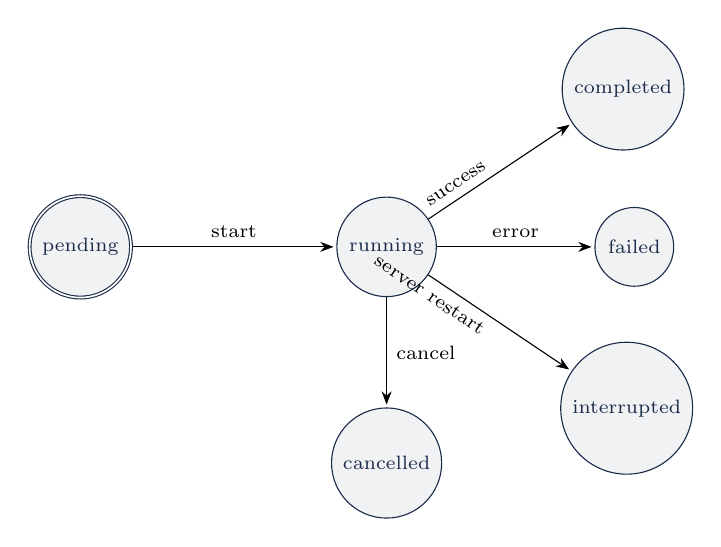
\begin{tikzpicture}[
  ->,>=Stealth,shorten >=1pt,auto,
  node distance=2.0cm,
  every state/.style={draw=fptNavy,fill=fptNavy!6,text=fptNavy,
                      minimum size=1.0cm,font=\scriptsize},
]
  \node[state,double] (pend) {pending};
  \node[state,right=2.6cm of pend]      (run)  {running};
  \node[state,above right=1.0cm and 2.0cm of run]  (done) {completed};
  \node[state,right=2.0cm of run]       (fail) {failed};
  \node[state,below right=1.0cm and 2.0cm of run]  (int)  {interrupted};
  \node[state,below=1.4cm of run]       (can)  {cancelled};

  \path (pend) edge node[above]{\scriptsize start}   (run)
        (run)  edge node[above left,sloped]{\scriptsize success} (done)
        (run)  edge node[above]{\scriptsize error}   (fail)
        (run)  edge node[right]{\scriptsize cancel}  (can)
        (run)  edge node[below left,sloped]{\scriptsize server restart} (int);
\end{tikzpicture}
\end{center}
{\scriptsize \texttt{src/infrastructure/job\_store.py} --- thread-safe JSON persistence,
atomic tmp+rename writes, stale jobs marked \textit{interrupted} on restart}
\end{frame}

% ── SLIDE 9: Screen Design ────────────────────────────────────────────────────
\begin{frame}[shrink=5]{7. Screen Design}
\begin{tabular}{@{}llp{5.2cm}@{}}
\toprule
\textbf{Interface} & \textbf{Technology} & \textbf{Key Features} \\
\midrule
Gradio Demo          & src/app\_gradio.py     & Interactive QA, real inference, no mocked responses \\
GraphPulse Dashboard & src/dashboard/         & SVG charts, query logs, KG stats, keyboard nav (\texttt{/} focus, Esc clear), focus-visible a11y \\
REST API             & FastAPI /query /ingest & OpenAPI docs, API key auth, rate limiting 120 req/min \\
MCP Server           & src/mcp\_pkg/          & Claude Desktop integration, 6 tools exposed \\
\bottomrule
\end{tabular}

\begin{exampleblock}{Real pipeline on every interface}
{\small All interfaces run the real NER$\to$embed$\to$WRRF$\to$rerank$\to$LLM
pipeline --- no fake or hard-coded demo paths.}
\end{exampleblock}
\end{frame}

% ── SLIDE 10: Technology Choices ──────────────────────────────────────────────
\begin{frame}[shrink=5]{8. Technology Choices}
\begin{tabular}{@{}llp{5.8cm}@{}}
\toprule
\textbf{Layer} & \textbf{Technology} & \textbf{Rationale} \\
\midrule
Backend      & FastAPI + Python 3.12             & Async, Pydantic v2, OpenAPI auto-docs \\
Graph DB     & Neo4j 5.x                         & Vector index + fulltext + Cypher in one DB \\
Embeddings   & GreenNode-Embedding-Large-VN      & Best MAP@5 for Vietnamese (1024-dim) \\
NER          & ViDeBERTa/wikilink --- 6 backends & Pluggable; wikilink best for bulk (F1=46.9\%) \\
Reranker     & BAAI/bge-reranker-v2-m3           & Cross-encoder, multilingual, no fine-tuning needed \\
LLM          & Vi-Qwen2-7B-RAG 4-bit NF4        & Local-first, Vietnamese-specific, quantized \\
Toolchain    & uv + ruff + mypy + pre-commit     & Modern Python: fast deps, lint, type-check \\
External APIs & Gemini · HuggingFace · Wikidata  & Embedding backup, dataset source, entity enrichment \\
\bottomrule
\end{tabular}
\end{frame}

% ── SLIDE 11: Coding Quality & Patterns ──────────────────────────────────────
\begin{frame}[shrink=5]{9. Coding Quality \& Design Patterns}
\begin{block}{Coding Conventions \checkmark}
\begin{itemize}\setlength\itemsep{1pt}\small
  \item ruff + ruff-format enforced via pre-commit hooks
  \item mypy strict type-checking
  \item CI runs lint + typecheck + test
  \item \texttt{snake\_case} / \texttt{SCREAMING\_SNAKE\_CASE} / \texttt{\_idx}/\texttt{\_ft} naming enforced
\end{itemize}
\end{block}

\begin{exampleblock}{Config \& Secrets \checkmark}
{\small All secrets via \texttt{pydantic\_settings.BaseSettings} from \texttt{.env}.
\texttt{.env.example} provided. No hard-coded credentials anywhere in source.}
\end{exampleblock}

\begin{tabular}{@{}llp{4.5cm}@{}}
\toprule
\textbf{Pattern} & \textbf{Applied In} & \textbf{Benefit} \\
\midrule
Strategy  & NER backends via \texttt{NER\_BACKEND} env & Swap NER without code change \\
Singleton & Neo4j driver · Local LLM lazy-load         & Single connection pool \\
Factory   & \texttt{get\_ner\_backend()}                & Decouple creation from use \\
Facade    & WRRF retrieval pipeline                    & Hides 4-signal complexity from agent \\
\bottomrule
\end{tabular}
\end{frame}

% ── SLIDE 12: Algorithm Complexity ───────────────────────────────────────────
\begin{frame}[shrink=8]{10. Algorithm Complexity}
\begin{alertblock}{Problem Definition}
{\small $Q \rightarrow$ retrieve $\{P_1 \ldots P_n\}$ from KG $G$
$\rightarrow$ generate $A$ + citations.
Complexity levels: 1-hop (lookup), 2-hop (bridge), 3-hop (fan-out).}
\end{alertblock}

\begin{tabular}{@{}lll@{}}
\toprule
\textbf{Algorithm} & \textbf{Purpose} & \textbf{Citation} \\
\midrule
WRRF 4-signal fusion    & BM25+Vector+Graph+Community     & Cormack et al. RRF \\
Leiden/Louvain          & Community detection              & Edge et al. 2024 \\
ReAct ($\leq$6 iter)    & Step-by-step graph reasoning     & Yao et al. 2023 \\
Multi-trajectory voting & Robust multi-hop ($N$ parallel)  & Thompson et al. 2025 \\
QLoRA ($r$=32)          & Text2Cypher fine-tuning          & Dettmers et al. 2023 \\
\bottomrule
\end{tabular}

\begin{block}{WRRF Formula}
\[
  \text{score}(d) = \sum_{i} \frac{w_i}{k + \text{rank}_i(d)} \quad k=60
\]
{\small $w_\text{BM25}=0.4,\ w_\text{Vector}=0.4,\ w_\text{Graph}=0.2,\
w_\text{Community}=0.15$. \quad
\pos{+20.8\% MRR vs best non-graph baseline \checkmark}}
\end{block}
\end{frame}

% ── SLIDE 13a: Corpus Filter Pipeline ────────────────────────────────────────
\begin{frame}[shrink=15]{11. Data Pipeline — Corpus Filtering}
\begin{columns}[T]
\column{0.52\textwidth}
\begin{block}{11-Stage Filter: \texttt{viwiki-20260501}}
\begin{tabular}{@{}lrr@{}}
\toprule
\textbf{Stage} & \textbf{Count} & \textbf{Drop} \\
\midrule
Initial dump        & 1{,}614{,}015 & --- \\
Redirect filter     & 1{,}300{,}130 & $-$313K \\
Disambiguation      & 1{,}284{,}671 & $-$15K \\
List pages          & 1{,}279{,}292 & $-$5K \\
Year/date pages     & 1{,}276{,}304 & $-$3K \\
Dup-line filter     & 1{,}275{,}171 & $-$1K \\
Word count pre      &   414{,}397 & $-$861K \\
Orphan filter       &   397{,}438 & $-$17K \\
Word count final    &   357{,}747 & $-$40K \\
Stop words          &   357{,}736 & $-$11 \\
Exact dedup         &   357{,}714 & $-$22 \\
\textbf{MinHash dedup} & \textbf{353{,}498} & $-$4K \\
\bottomrule
\end{tabular}
\end{block}

\column{0.44\textwidth}
\begin{exampleblock}{Key Design Choices}
\begin{itemize}\scriptsize\setlength\itemsep{2pt}
  \item Word count pre-filter: largest single drop ($-$861K stubs)
  \item Orphan filter: removes unlinked articles ($-$17K)
  \item MinHash dedup: Jaccard $\geq 0.85$ threshold
  \item \textbf{No} punctuation-ratio filter: Wikipedia tables/lists naturally break the 60\% threshold; dropped after analysis
\end{itemize}
\end{exampleblock}

\begin{block}{Result}
{\small $1{,}614{,}015 \rightarrow$ \pos{\textbf{353{,}498}} articles\\
(21.9\% of original dump retained)\\
Snapshot: \texttt{viwiki-20260501}}
\end{block}
\end{columns}
\end{frame}

% ── SLIDE 13b: ViWikiHop Schema ───────────────────────────────────────────────
\begin{frame}[shrink=20]{12. Data Pipeline — ViWikiHop Schema v0.4}
\begin{columns}[T]
\column{0.50\textwidth}
\begin{block}{Entry Schema (schema v0.4)}
{\scriptsize
\begin{tabular}{@{}lp{3.2cm}@{}}
\toprule
\textbf{Field} & \textbf{Description} \\
\midrule
\texttt{\_id}           & \texttt{hw-} / \texttt{syn-mh-} / \texttt{uvq-} \\
\texttt{question}       & Vietnamese question \\
\texttt{answer}         & Empty if unanswerable \\
\texttt{supporting\_facts} & Evidence refs \\
\texttt{context}        & Paragraph segments \\
\texttt{type}           & 8 reasoning types \\
\texttt{level}          & easy / medium / hard \\
\texttt{source}         & 3 sources \\
\texttt{num\_hops}      & $\geq 1$ \\
\texttt{is\_vi\_exclusive} & VI-exclusive track \\
\texttt{is\_impossible} & Unanswerable flag \\
\texttt{decomposition}  & Sub-Q/A per hop \\
\texttt{plausible\_answer} & For unanswerable only \\
\bottomrule
\end{tabular}
}
\end{block}

\column{0.46\textwidth}
\begin{block}{3 Data Sources}
\begin{tabular}{@{}ll@{}}
\toprule
\textbf{Source} & \textbf{Description} \\
\midrule
\texttt{hw-}      & Human annotated \\
\texttt{syn-mh-}  & KG walk synthesis \\
\texttt{uvq-}     & ViQuAD 2.0 import \\
\bottomrule
\end{tabular}
\end{block}

\begin{alertblock}{Schema v0.4 Key Invariants}
\begin{itemize}\scriptsize\setlength\itemsep{2pt}
  \item Single-hop: \texttt{decomposition} = $[\,]$
  \item Unanswerable: \texttt{answer}=\texttt{""}, non-empty \texttt{plausible\_answer}
  \item Multi-hop: $|\texttt{decomposition}|$ = \texttt{num\_hops}
  \item UIT-ViQuAD: \texttt{is\_vi\_exclusive} always false
\end{itemize}
\end{alertblock}
\end{columns}
\end{frame}

% ── SLIDE 13c: Reasoning Types & Difficulty ───────────────────────────────────
\begin{frame}[shrink=15]{13. Data Pipeline — Reasoning Types \& Difficulty}
\begin{columns}[T]
\column{0.50\textwidth}
\begin{block}{8 Reasoning Types}
\begin{tabular}{@{}lp{3.5cm}@{}}
\toprule
\textbf{Type} & \textbf{Description} \\
\midrule
\texttt{lookup}        & One article, one fact \\
\texttt{bridge}        & A $\to$ bridge entity $\to$ B \\
\texttt{comparison}    & Compare $\geq 2$ article values \\
\texttt{intersection}  & Entity from $\geq 2$ constraints \\
\texttt{temporal}      & Date order / chronology \\
\texttt{numerical}     & Arithmetic or counting \\
\texttt{fan-out}       & Aggregate related entities \\
\texttt{unanswerable}  & No valid answer in context \\
\bottomrule
\end{tabular}
\end{block}

\column{0.46\textwidth}
\begin{block}{3-D Difficulty Rubric}
{\small Score = hop\_count + lexical\_overlap + reasoning\_op}\\[4pt]
\begin{tabular}{@{}lccc@{}}
\toprule
\textbf{Score} & \textbf{Hop} & \textbf{Lexical} & \textbf{ReasonOp} \\
\midrule
0 & 1-hop     & $\geq 60\%$ & lookup \\
1 & 2-hop     & 30--60\%    & bridge/comparison \\
2 & $\geq$3-hop & $< 30\%$ & temporal/numerical/\ldots \\
\bottomrule
\end{tabular}

\vspace{4pt}
\begin{tabular}{@{}ll@{}}
\toprule
\textbf{Total (0--6)} & \textbf{Level} \\
\midrule
0--1 & \HL{easy} \\
2--3 & \con{medium} \\
4--6 & \pos{hard} \\
\bottomrule
\end{tabular}
\end{block}
\end{columns}
\end{frame}

% ── SLIDE 13d: QA Generation & QC Pipeline ────────────────────────────────────
\begin{frame}[shrink=10]{14. Data Pipeline — QA Generation \& QC}
\begin{columns}[T]
\column{0.50\textwidth}
\begin{block}{QA Generation Pipeline}
\begin{enumerate}\small\setlength\itemsep{3pt}
  \item \textbf{Bridge Extraction} --- follow \texttt{[[wikilinks]]} to build article-pair bridges; no Neo4j walk
  \item \textbf{LLM Sampling} --- prompt LLM to generate questions directly from bridge pairs (no templates)
  \item \textbf{Labelling} --- \textbf{Gemini 2.5 Flash Lite} reads difficulty rubric and assigns type + level
  \item \textbf{Verification} --- \textbf{DeepSeek V3 Pro} independently verifies label and answer grounding
\end{enumerate}
\end{block}

\begin{exampleblock}{Sample Entry ID}
{\scriptsize \texttt{syn-mh-viex-b1-a-00001}\\
type=bridge, level=medium, num\_hops=2\\
is\_vi\_exclusive=true, source=synthetic-multihop}
\end{exampleblock}

\column{0.46\textwidth}
\begin{block}{Two-Model QC Gate}
\begin{tabular}{@{}lp{2.8cm}@{}}
\toprule
\textbf{Model} & \textbf{Role} \\
\midrule
Gemini 2.5 Flash Lite & Label (type, level, decomposition) \\
DeepSeek V3 Pro       & Verify label + grounding \\
\bottomrule
\end{tabular}
\smallskip

{\scriptsize Gate logic: entry passes only when both models agree on answer grounding; label is taken from Gemini, rejected if DeepSeek flags a mismatch.}
\end{block}

\begin{block}{Schema QC (post-gate)}
\begin{itemize}\scriptsize\setlength\itemsep{1pt}
  \item Well-formedness: non-empty fields, schema v0.4
  \item Grounding: answer in supporting\_facts verbatim
  \item Natural phrasing: no \textit{``Theo bài viết''} phrases
  \item Dedup: exact + MinHash ($J \geq 0.85$)
\end{itemize}
\end{block}
\end{columns}
\end{frame}

\iffalse
% ── SLIDE 14: Model Training ──────────────────────────────────────────────────
\begin{frame}[shrink=15]{15. Model Training (QLoRA)}
\begin{columns}[T]
\column{0.48\textwidth}
\begin{block}{QLoRA Fine-tuning --- Text2Cypher}
{\scriptsize
\begin{tabular}{@{}ll@{}}
\toprule
\textbf{Param} & \textbf{Value} \\
\midrule
Base model      & Vi-Qwen2-7B-RAG \\
Quant           & 4-bit NF4 \\
LoRA $r$        & 32 \\
lora\_alpha     & 64 \\
lora\_dropout   & 0.05 \\
Target modules  & q\_proj, v\_proj \\
Epochs          & 3 \\
\bottomrule
\end{tabular}
}
\smallskip\\
{\scriptsize Adapter: \texttt{LORA\_ADAPTER\_PATH}, lazy-loaded at first query}
\end{block}

\column{0.48\textwidth}
\begin{block}{Transfer Learning (pre-trained)}
{\scriptsize
\begin{tabular}{@{}p{2.8cm}p{2.8cm}@{}}
\toprule
\textbf{Model} & \textbf{Role} \\
\midrule
GreenNode-VN        & Dense embeddings \\
ViDeBERTa (electra) & NER (F1=44\%) \\
BGE-reranker-v2-m3  & Cross-encoder rerank \\
Vi-Qwen2-7B-RAG     & Answer generation \\
\bottomrule
\end{tabular}
}
\end{block}
\end{columns}
\end{frame}

% ── SLIDE 15: Evaluation Results ─────────────────────────────────────────────
\begin{frame}[shrink=8]{16. Evaluation Results}
\textbf{Baseline Comparison (ViQuAD2)}\\[4pt]
\begin{tabular}{@{}llll@{}}
\toprule
\textbf{Method} & \textbf{MRR} & \textbf{Hit@5} & \textbf{Latency} \\
\midrule
BM25 only                         & ${\sim}0.35$ & ${\sim}55$\%   & 0.8s \\
Dense only                        & ${\sim}0.40$ & ${\sim}60$\%   & 1.2s \\
Naive RAG                         & ${\sim}0.42$ & ${\sim}62$\%   & 2.5s \\
BM25 + Vector                     & ${\sim}0.48$ & ${\sim}66$\%   & 1.5s \\
\pos{\textbf{Ours (WRRF+Rerank)}} & \pos{\textbf{0.4497}} & \pos{\textbf{64.67\%}} & \pos{\textbf{51ms}} \\
\bottomrule
\end{tabular}

\vspace{6pt}
\textbf{Multi-metric (ViQuAD2, 500 samples)}\\[4pt]
\begin{tabular}{@{}lll@{}}
\toprule
\textbf{Metric} & \textbf{Value} & \textbf{Notes} \\
\midrule
Context Hit Rate  & 0.726   & Top-5 recall \\
MRR               & 0.364   & Mean reciprocal rank \\
Token F1          & 0.1195  & Answer quality \\
NER F1 (wikilink) & 46.9\%  & Typed entity F1 \\
\bottomrule
\end{tabular}

\begin{alertblock}{Known Failure Modes}
\begin{itemize}\scriptsize\setlength\itemsep{1pt}
  \item abstain\_accuracy = 0.0 (model never abstains)
  \item Low hit rate on 3-hop fan-out (multi-entity gap)
  \item ${\sim}5$\% diacritic mismatch in entity resolution
\end{itemize}
\end{alertblock}
\end{frame}

% ── SLIDE 16: AI Engineering Quality ─────────────────────────────────────────
\begin{frame}[shrink=5]{17. AI Engineering Quality}
\begin{exampleblock}{No Fake Demo \checkmark}
{\small Full NER$\to$embed$\to$WRRF$\to$rerank$\to$LLM pipeline fires on every query.
Gradio, \texttt{/query} endpoint, dashboard, MCP all call real inference.}
\end{exampleblock}

\begin{block}{Custom Engineering (beyond plain API calls)}
\begin{itemize}\small\setlength\itemsep{1pt}
  \item WRRF 4-signal fusion with configurable weights
  \item Leiden community detection + summary retrieval (4th signal)
  \item Question complexity routing (simple/complex)
  \item Multi-trajectory majority vote ($N$ parallel)
  \item Vietnamese entity resolution (diacritic norm + alias merge)
  \item Cypher safety validation (write-keyword blocklist)
  \item QLoRA fine-tuning for Text2Cypher
  \item Multi-key Gemini rotation + exponential backoff
\end{itemize}
\end{block}

\begin{alertblock}{Gap: Experiment Tracking}
{\small No MLflow/W\&B/DVC. Eval results saved as timestamped JSON in
\texttt{reports/eval/}. MLflow integration planned for Week 9.}
\end{alertblock}
\end{frame}
\fi

% ── SLIDE 17: Team & Timeline ─────────────────────────────────────────────────
\begin{frame}[shrink=5]{18. Team Contribution \& Timeline}
\begin{tabular}{@{}llp{6.0cm}@{}}
\toprule
\textbf{Member} & \textbf{ID} & \textbf{Modules} \\
\midrule
Huynh Quoc Trung   & QE180038 & KG construction · NER (6 backends) · entity resolution · dataset gen \\
Nhu Quang Anh      & QE180005 & WRRF retrieval · reranker · evaluation pipeline · SRS docs \\
Pham Ngo Dinh Khoi & QE180110 & ReAct agent · local LLM · MHQA dataset · QLoRA fine-tuning \\
Truong Dinh Thien  & QE180018 & FastAPI · job management · Gradio demo · dashboard \\
\bottomrule
\end{tabular}

\vspace{4pt}
\begin{tabular}{@{}lll@{}}
\toprule
\textbf{Milestone} & \textbf{R1 Status} & \textbf{R2 Status} \\
\midrule
Core pipeline + SRS        & \pos{Done \checkmark}  & \pos{Stable \checkmark} \\
Full ingestion + ablation  & \con{In progress}      & \pos{Done \checkmark} \\
QLoRA Text2Cypher          & Pending                & \con{In progress} \\
WRRF tuning + final eval   & Pending                & \con{In progress} \\
Final report + defense     & Pending                & Pending \\
\bottomrule
\end{tabular}

\begin{block}{}
{\small UCP = 96.5 (UUCP=134 · TCF=0.9 · ECF=0.8) $\rightarrow$ On schedule \pos{\checkmark}}
\end{block}
\end{frame}

% ── SLIDE 18: Thank You ───────────────────────────────────────────────────────
\begin{frame}[plain]
\begin{center}
{\Huge \textbf{Thank You}}\\[12pt]
{\Large Q\&A}\\[8pt]
{\normalsize Vietnamese GraphRAG --- Multi-hop QA}
\end{center}
\end{frame}

% ─────────────────────────────────────────────────────────────────────────────
% APPENDIX
% ─────────────────────────────────────────────────────────────────────────────
\backupbegin

% A1: NER Backend Comparison
\begin{frame}[shrink=5]{Appendix: NER Backend Comparison}
\begin{tabular}{@{}lllp{4.2cm}@{}}
\toprule
\textbf{Backend} & \textbf{Typed F1} & \textbf{Speed} & \textbf{Notes} \\
\midrule
simple      & ${\sim}20$\%  & Fast    & Regex + keyword, no ML \\
underthesea & ${\sim}35$\%  & Medium  & BIO tagging, general Vietnamese \\
phonlp      & ${\sim}38$\%  & Slow    & PhoNLP + VnCoreNLP segmentation \\
phobert     & ${\sim}42$\%  & Slow    & PhoBERT transformer pipeline \\
videberta   & 44\%          & Medium  & ViDeBERTa/NlpHUST electra-base \\
wikilink    & \pos{46.9\%}  & Fast    & Wikipedia hyperlinks, best for bulk \\
\bottomrule
\end{tabular}
\end{frame}

% A2: WRRF Detail & Ablation
\begin{frame}[shrink=5]{Appendix: WRRF Detail \& Ablation}
\[
  \text{score}(d) = \sum_{i \in S} \frac{w_i}{k + \text{rank}_i(d)}
  \quad k=60,\quad \sum w_i \approx 1.15
\]

\begin{tabular}{@{}lllll@{}}
\toprule
\textbf{Variant} & \textbf{Signals} & \textbf{MRR} & \textbf{Hit@5} & \textbf{$\Delta$ MRR} \\
\midrule
BM25 only         & 1 & 0.35  & 55\%   & baseline \\
+ Vector          & 2 & 0.40  & 60\%   & +14.3\% \\
+ Graph           & 3 & 0.43  & 63\%   & +22.9\% \\
\pos{+ Community} & \pos{4} & \pos{0.4497} & \pos{64.67\%} & \pos{+28.5\%} \\
\bottomrule
\end{tabular}
\end{frame}

% A3: MHQA Generation Pipeline
\begin{frame}{Appendix: MHQA Generation Pipeline}
\begin{enumerate}\small\setlength\itemsep{3pt}
  \item \textbf{KG Walk Extraction} --- 2-hop, 3-hop, and broken-link walks from Neo4j
    (\texttt{scripts/mhqa\_extract\_walks.py})
  \item \textbf{Template QA Generation} --- Vietnamese question templates instantiated
    from walk triples (\texttt{scripts/mhqa\_generate.py})
  \item \textbf{LLM Rewrite} --- Optional naturalness rewrite via Gemini
    (\texttt{scripts/mhqa\_generate.py --rewrite})
  \item \textbf{5-Stage QC Pipeline} (\texttt{scripts/mhqa\_qc.py}):
    \begin{enumerate}\scriptsize
      \item Well-formedness (length, punctuation, Vietnamese chars)
      \item Grounding (\texttt{entity\_grounded\_in\_text} verification)
      \item Deduplication (MinHash + exact match)
      \item Answerability (answer appears in supporting chunk)
      \item Schema validation (required fields present)
    \end{enumerate}
  \item \textbf{Retrievability Check} (\texttt{scripts/mhqa\_retrievability.py}) ---
    confirms each QA pair is retrievable by WRRF pipeline before inclusion
\end{enumerate}
\end{frame}

\backupend

\end{document}
